%=============================================================================
% Thesis Template in LaTex
%
% File:  07-Schlussfolgerung.tex -- Schlussfolgerung und Ausblick
% Author(s): Cyrano Golliez <golliezc@student.ethz.ch>
%
% Creation:  27 Jan 2014
% Time-stamp: <Tue 2013-08-13 20:14 juergen>
%
% Copyright (c) 2014 Infrastructure Management Group (IMG)
%               http://ibi.ethz.ch
%
% More information on LaTeX: http://www.latex-project.org/
%=============================================================================

\chapter{Schlussfolgerung und Ausblick}
\label{chap:Schlussfolgerung}




Eine Aufteilung der Kosten nach den verschiedenen Interessensverbänden wäre im Rahmen der Diskussion sehr aufschlussreich gewesen. Da die die Situation und die Möglichkeiten die mir für die Modellierung zur Verfügung standen zur Folge haben, dass die Reisezeitkosten den gesamten Risikovergleich der Varianten bestimmten, habe ich im Rahmen der Diskussion der Ergebnisse auf diese Unterteilung verzichtet. Es wäre jedoch sehr interessant, im Rahmen der weiteren Prüfung der Varianten, eine vertieftere Beurteilung der Nutzer- und Besitzerkosten durchzuführen.

Der Vergleich der Reisezeitkosten ist das ausschlaggebende Argument der Variante 2. In der Diskussion wurde die Mehrkosten
Mehrkosten Reisezeit -> V1 vs V2 übersteigen höher bau und wartungskosten umeinvielfaaches.,.. somit wäre nicht nur nachhaltig und ökologisch sondern auch ökonisch die beste option.!! 


Hinsichtlich der zukünftigen Entwicklung der Mobilität wird das Fahrrad vorraussichtlich auch auf Strecken bis zu 30km eine entscheidende Rolle bei der Verkehrsmittelwahl spielen. Aufgrund dessen und in anbetracht der Bestrebungen der Stadt Uster ein Zentrum mit regionaler Bedeutung zu werden, ist die Förderung des ökologischen und zukunftsorientierten Langsamverkehrs unerlässlich und insbesondere im Rahmen einer nachhaltigen Stadtentwicklung voranzutreiben.

Somit kann die geplante Veloroute eine Reduktion der Belastung der Öffentlichkeit, in Form der Reduktion der Schadstoffemission, erreichen. 	
Die Schwierigkeit diese Kosten zu modelieren liegt in der nicht direkt messbaren Beziehung zwischen Schadstoffbelastung und daraus resultierenden Kosten. Jedoch ist zu vermerken das die Emissionen direkt von der Anzahl an motorisierten Fahrzeuge abhängt die auf der Infrastruktur verkehren.

%Das Ziel dieser Infrastruktur ist es grössere Distanzen in kurzer Zeit und mit hoher Geschwindigkeit unmotorisiert zurück legen zu könne. Dies setzt eine kreuzungsfreie Ausführung vorraus was mit baulichen Massnahmen oder Vortrittsberechtigungen erreicht werden kann.

ausblick: mögliche erweiterung der Veloinfrastruktur bis zum Nüslikreisel oder bis zum Spital... Die Infrastrukturintervention wäre ein Ausbau der Nord-Süd Achse entlang der Pfäffikerstrasse, Brunnen- und Bahnhofstrasse zu einer Veloschnellstrasse. Das Vorbild dieser Infrastruktur ist die C99, Kopenhagen-Albertslund eine sogenannten \textit{Super-Radschnellroute} auch bekannt als \textit{Cykelsuperstier}. Diese Art von Veloinfrastruktur hat sich bereits in Dänemark bewehrt um das Pendeln leichter und sicherer zu machen. 

%In Anbetracht der enormen Kapazitätssteigerung wäre ein Ausbau der Parkplätze auf der Sportanlage Buchenholz zu prüfen. Dies wäre im Rahmen eines Programmes gedacht das sich \textit{Ride and Bike} nennen könnte, welches zum Ziel hat die Kombination von Autobahnanschluss und Parkiermöglichkeit mit einer bequemen, sicheren und schnellen Veloverbindung ins Stadtzentrum zu fördern.

Die von mir vorgeschlagenen Schritte die Uster in der nächsten Zeit tätigen soll oder kann sind in der nachfolgenden Abbildung \ref{img:UsterFuture} dargestellt. \\
So ergibt sich einerseits, wie ausführlich besprochen, der Weg die Variante 2 in Betracht zu ziehen und die weitere Schritte dementsprechend einzuleiten, wie zum Beispiel der Beginn einer Detailstudie oder aber bereits der Start des Planungsprozesses. Der zweite Weg der sich der Stadt Uster bietet, ist eine weitere Hauptstudie, wodurch infolge der ausführlichen Prüfung der Situation, entweder die Wahl der optimalen Variante manifestiert oder aber eine andere Variante als die als optimal zu erachtende Variante bestimmt wird. Die letzte Möglichkeit die sich der Stadt Uster bietet, ist die Option: Variante 1 - "nichts zu machen", wobei für relativ wenig Geld die Verkehrssicherheit marginal erhöht wird. 

\begin{figure}[h!]
	\centering
	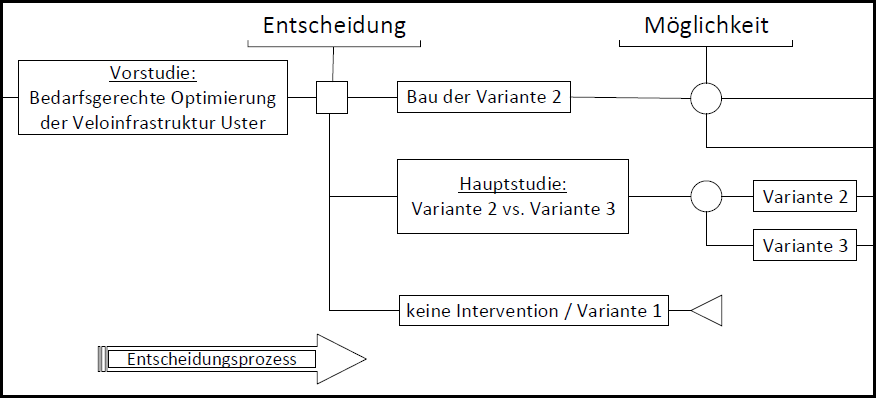
\includegraphics[width=.45\textwidth]{figures/f-07-01-EntscheidungsprozessUster}
	\caption[Entscheidungsprozess der Stadt Uster]{Möglicher Entscheidungsprozess der Stadt Uster für die nähere Zukunft}
	\label{img:UsterFuture}
\end{figure} 

\paragraph{Ausblick}

Das betrachtete Problemfeld der im Rahmen dieser Projektarbeit gestellten Aufgabenstellung ist sehr umfangreich. Um ein ansprechendes Resultat im gegebenen Zeitrahmen erarbeiten zu können, mussten einige Vereinfachungen und Annahmen gemacht und ein Schwerpunkt auf ein System gelegt werden. Es hätten demnach einige weiter Punkte berücksichtigt sowie gewisse Akspekte genauer modelliert werden können. \\
So hätten zum einen die Interessensgruppe der Nutzer differenzierter betrachtet und um die Fussgänger erweitert werden können. Im gleichen Zuge hätte der Öffentliche Verkehr in die Entscheidungsfindung miteinbezogen werden müssen, was in Anbetracht dessen, dass der Bahnübergang Brunnenstrasse im Busnezt ein zentraler Knotenpunkt ist, in einer vollumfänglichen Betrachtung der Situation unerlässich ist. Zusätzlich hätten politische Entscheidungen sowie Budgetgrenzen der Stadt Uster und des Kantons Zürich berücksichtigt werden können, um eine politisch tragbare und realitätsnahe optimale Variante erarbeiten zu können.

Um eine genauere Vorhersage der Zukunft von Uster machen zu können, wäre das Berücksichtigen weiterer Szenarien und demnach weitere Einflussfaktoren notwendig. Durch die Berücksichtigung weiterer Einflussfaktoren wird die Modellierung der Parameter sowie die Risikoberechnung der Varianten komplizierter jedoch das Resultat der Optimierung exakter. 
So wäre eine Verkehrssimulation, mit der die effektive Verkehrslage in der Stadt modelliert wird, ein geeignetes Mittel, um zum Beispiel im Falle der Variante 3 die entstehende Wartezeit aufgrund des Ampelsystems genauer zu bestimmen. Mithilfe von Verkehrssimulation wäre demnach ein exakteres Resultat zu erwarten und die Infrastruktur der Varianten könnte auf ihre Gebrauchstauglichkeit untersucht werden. Zusättzlich wäre das Modellieren der Verkehrssicherheit der verschiedenen Varianten ein wichtiger Schritt, um die effektive Gefahrenlage, die von einer jeweiligen Variante ausgeht, in die Wahl der optimalen Variante miteinzubeziehen.\\
Und abschliessend wäre 
  



% ===========================================================================
% EOF
%

%%% Local Variables:
%%% mode: latex
%%% TeX-master: "../main"
%%% End:
